%% Presentation for KES 2026
%% Paper: Agentic AI for Public Administration:
%%        A Multi-Agent Architecture and Controlled Fault Injection Evaluation
%%
%% Layout follows the structure of KES26-model.pdf in this directory
%% (part dividers, block-driven slides, three-cell footline), with its own
%% palette: deep teal, slate, rust.
%%
%% Compile with: pdflatex KES26-Radu.tex   (run twice, for the frame counter)

\documentclass[aspectratio=169,10pt]{beamer}

\usetheme{default}
\usepackage[T1]{fontenc}
\usepackage{lmodern}
\usepackage{booktabs}
\usepackage{graphicx}
\usepackage{amsmath}
\usepackage{amssymb}
\usepackage{xcolor}
\usepackage{tikz}
\usetikzlibrary{arrows.meta, positioning}

\graphicspath{{../figures/}}

%% ---------------------------------------------------------------- palette --
\definecolor{teal}{RGB}{13,78,85}      % primary: title bar, structure, emphasis
\definecolor{slate}{RGB}{58,66,86}     % block headers
\definecolor{rust}{RGB}{158,68,32}     % alert headers, risk emphasis
\definecolor{mist}{RGB}{242,244,245}   % block bodies
\definecolor{stone}{RGB}{110,116,122}  % captions, footline

\setbeamercolor{structure}{fg=teal}
\setbeamercolor{alerted text}{fg=rust}
\setbeamercolor{frametitle}{bg=teal, fg=white}
\setbeamercolor{footline}{fg=stone}
\setbeamercolor{block title}{bg=slate, fg=white}
\setbeamercolor{block body}{bg=mist, fg=black}
\setbeamercolor{block title alerted}{bg=rust, fg=white}
\setbeamercolor{block body alerted}{bg=mist, fg=black}
\setbeamercolor{block title example}{bg=teal, fg=white}
\setbeamercolor{block body example}{bg=mist, fg=black}
\setbeamercolor{itemize item}{fg=teal}
\setbeamercolor{itemize subitem}{fg=teal}
\setbeamercolor{enumerate item}{fg=teal}

\setbeamertemplate{blocks}[default]
\setbeamertemplate{navigation symbols}{}
\setbeamertemplate{itemize items}[square]
\setbeamertemplate{itemize subitem}[square]

\setbeamerfont{frametitle}{size=\large, series=\bfseries}
\setbeamerfont{block title}{size=\small, series=\bfseries}
\setbeamerfont{footline}{size=\tiny}

%% ------------------------------------------------- frame title and footer --
\setbeamertemplate{frametitle}{%
  \nointerlineskip%
  \begin{beamercolorbox}[wd=\paperwidth, ht=3.0ex, dp=1.6ex,
                         leftskip=0.30cm, rightskip=0.30cm]{frametitle}%
    \usebeamerfont{frametitle}\insertframetitle%
  \end{beamercolorbox}%
}

\newif\ifbackupslide
\setbeamertemplate{footline}{%
  \hbox{%
    \begin{beamercolorbox}[wd=0.34\paperwidth, ht=2.6ex, dp=1.4ex,
                           leftskip=0.30cm]{footline}%
      \usebeamerfont{footline}\insertshorttitle{} $\cdot$ KES 2026%
    \end{beamercolorbox}%
    \begin{beamercolorbox}[wd=0.32\paperwidth, ht=2.6ex, dp=1.4ex,
                           center]{footline}%
      \usebeamerfont{footline}\insertsection%
    \end{beamercolorbox}%
    \begin{beamercolorbox}[wd=0.34\paperwidth, ht=2.6ex, dp=1.4ex,
                           rightskip=0.30cm]{footline}%
      \usebeamerfont{footline}\hfill
      \ifbackupslide backup\else\insertframenumber/\inserttotalframenumber\fi%
    \end{beamercolorbox}%
  }%
}

%% -------------------------------------------------------- small utilities --
\newcommand{\hl}[1]{\textcolor{teal}{\textbf{#1}}}      % emphasis
\newcommand{\risk}[1]{\textcolor{rust}{\textbf{#1}}}    % failure, silent rate
\newcommand{\cmt}[1]{{\color{stone}\small #1}}          % caption under content

% part divider
\newcommand{\keypart}[2]{%
  \begin{frame}[plain, noframenumbering]
    \vfill
    \centering
    {\color{stone}\small #1}\\[0.35em]
    {\color{teal}\Large\bfseries #2}\\[0.9em]
    {\color{rust}\rule{0.25\paperwidth}{1.2pt}}
    \vfill\vfill
  \end{frame}%
}

%% ------------------------------------------------------------------ title --
\title[Agentic AI for Public Administration]{Agentic AI for Public Administration}
\author{Radu-Mihai Gheorghe, Petru-Liviu Bouruc, Ciprian Paduraru, Alin Stefanescu}
\date{KES 2026}

\begin{document}

%% ================================================================== title ==
\begin{frame}[plain, noframenumbering]
  \vfill
  \centering
  {\color{teal}\large\bfseries
   Agentic AI for Public Administration:\\[0.15em]
   A Multi-Agent Architecture and\\[0.15em]
   Controlled Fault Injection Evaluation}\\[0.8em]
  {\color{rust}\rule{0.42\paperwidth}{1pt}}\\[1.1em]

  Radu-Mihai Gheorghe$^{1,2}$ \quad Petru-Liviu Bouruc$^{2}$ \quad
  Ciprian Paduraru$^{2}$ \quad Alin Stefanescu$^{2,3}$\\[0.9em]

  {\footnotesize $^{1}$UiPath, Romania}\\[0.3em]
  {\footnotesize $^{2}$University of Bucharest, Romania}\\[0.3em]
  {\footnotesize $^{3}$Institute for Logic and Data Science, Romania}\\[1.2em]

  30th International Conference on Knowledge-Based and\\
  Intelligent Information \& Engineering Systems (KES 2026)\\[1.1em]

  {\color{stone}\footnotesize Artifact:
   \texttt{github.com/radugheo/agentic-public-administration}}
  \vfill
\end{frame}

%% ============================================================== PART 1 ======
\keypart{PART 1}{Motivation}
\section{Motivation}

\begin{frame}{The fragmentation problem}
  Romania's fiscal services are spread over three national portals, each with its own
  interface, vocabulary and procedural logic:
  \begin{itemize}
    \item \textbf{SPV}, \emph{Spa\c{t}iul Privat Virtual} (Virtual Private Space): filing
      declarations, consulting your fiscal record
    \item \textbf{Ghi\c{s}eul.ro}, from \emph{ghi\c{s}eu} (service counter): paying taxes and
      contributions
    \item \textbf{RO e-Factura}: national electronic invoicing
  \end{itemize}
  \vfill
  In one year a freelancer declares annual income, pays pension and health contributions,
  registers a rental contract and issues an invoice, across portals sharing no state.
  \vfill
  \begin{block}{Where the burden sits}
    Computing the amounts is simple arithmetic. The effort goes into \hl{which declaration
    applies, under which deadline, on which portal}, and the rules that settle each.
  \end{block}
\end{frame}

\begin{frame}{A concrete request}
  \begin{columns}[T]
    \begin{column}{0.47\textwidth}
      \textbf{The task}\\[0.3em]
      \emph{``I earned 150,000 RON as a freelancer last year. What do I owe?''}
      \smallskip

      {\small Three amounts, under the 2026 rules, on a minimum gross salary of 4,050 RON:}
      \smallskip

      {\footnotesize
      \begin{tabular}{@{}llr@{}}
        \toprule
        \textbf{CAS} pension  & 25\% of $24\times4{,}050$ & 24,300\\
        \textbf{CASS} health  & 10\% of 150,000           & 15,000\\
        \textbf{Impozit} tax  & 10\% of 110,700           & 11,070\\
        \midrule
        \multicolumn{2}{@{}l}{\textbf{Total}} & \hl{50,370}\\
        \bottomrule
      \end{tabular}}

    \end{column}
    \begin{column}{0.47\textwidth}
      \centering
      \textbf{What the citizen never sees}\\[0.6em]
      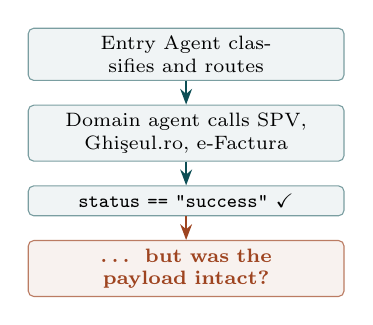
\begin{tikzpicture}[node distance=3mm, every node/.style={font=\scriptsize},
          b/.style={draw=teal!55, fill=teal!6, rounded corners=2pt, align=center,
                    inner sep=3pt, text width=38mm},
          ar/.style={-{Stealth[length=2mm]}, draw=teal, line width=0.7pt}]
        \node[b] (r) {Entry Agent classifies and routes};
        \node[b, below=of r] (a) {Domain agent calls SPV, Ghi\c{s}eul.ro, e-Factura};
        \node[b, below=of a] (s) {\texttt{status == "success"} \checkmark};
        \node[b, below=of s, draw=rust!70, fill=rust!7] (v)
             {\risk{\ldots{} but was the payload intact?}};
        \draw[ar] (r) -- (a); \draw[ar] (a) -- (s);
        \draw[ar, draw=rust] (s) -- (v);
      \end{tikzpicture}
    \end{column}
  \end{columns}
\end{frame}

\begin{frame}{What this paper does}
  \begin{block}{Build}
    \small A multi-agent assistant for Romanian tax and fiscal administration. An Entry Agent
    classifies the citizen's request and routes it to one of five domain agents, over four
    shared services, built with UiPath Coded Agents on LangGraph: D212 filing, property sale,
    rental income, fiscal certificates and RO e-Factura.
  \end{block}
  \begin{block}{Break}
    \small Every call the assistant makes into SPV, Ghi\c{s}eul.ro and e-Factura is instrumented
    with four chaos operators: timeout, delay, partial response and corruption, at a
    configurable rate, replayable from a seed.
  \end{block}
  \begin{block}{Measure}
    \small For each injected fault, look at the answer the citizen actually receives. Did the
    failure surface, or did it pass through silently?
  \end{block}
\end{frame}

\begin{frame}{Research questions}
  \begin{block}{RQ1 \quad How much gets through?}
    When a service behind the assistant is slow, returns an incomplete payload or a corrupted
    one, \hl{what fraction of those faults reaches the citizen with no signal at all}, in an
    answer that reads as a normal success?
  \end{block}
  \vfill
  \begin{block}{RQ2 \quad Is that rate incidental, or structural?}
    Is the fraction a property of this implementation, to be driven down by better engineering,
    or is it \hl{fixed by the shape of the response schema and the predicate the agent branches
    on}, and therefore predictable before the system is ever run?
  \end{block}
\end{frame}

%% ============================================================== PART 2 ======
\keypart{PART 2}{The system}
\section{The system}

\begin{frame}{How the system is organised}
  \begin{columns}[T]
    \begin{column}{0.48\textwidth}
      \begin{block}{The Entry Agent}
        \small Every request enters here. The agent classifies it into intent, confidence,
        reasoning and extracted entities. A fixed table maps intent to a graph node, and low
        confidence diverts to clarification.
      \end{block}
      \begin{block}{Five domain agents}
        \small PFA/freelancer (D212), property sale, rental income, fiscal certificate and
        RO e-Factura. Each one reads the shared state, calls the shared services and writes
        the state back.
      \end{block}
    \end{column}
    \begin{column}{0.48\textwidth}
      \begin{block}{Four shared services}
        \small Document intake (OCR and schema validation), RAG over the Romanian Tax Code,
        deterministic calculation in decimal arithmetic, and payment through Ghi\c{s}eul.ro.
      \end{block}
      \begin{block}{Infrastructure: UiPath Coded Agents}
        \small One environment for model access, retrieval indices, storage buckets and human
        review tasks, so none of it has to be assembled separately.
      \end{block}
    \end{column}
  \end{columns}
  \vfill
  \cmt{Hierarchical supervisor pattern, implemented as a LangGraph \texttt{StateGraph} with
  typed shared state and conditional routing.}
\end{frame}

\begin{frame}{What the UiPath platform provides}
  A bare LangGraph implementation still leaves model access, retrieval infrastructure,
  escalation and document storage to be assembled separately. Here they come from one
  execution environment.
  \vfill
  {\small
  \begin{tabular}{@{}ll@{}}
    \toprule
    \textbf{Concern} & \textbf{UiPath resource}\\
    \midrule
    Model access                 & LLM Gateway, serving GPT-4o\\
    Grounding in the Tax Code    & Context Grounding indices, one per domain\\
    Document storage             & Storage buckets\\
    Human escalation             & Action Center tasks\\
    \bottomrule
  \end{tabular}}
  \vfill
  \centering
  Built with \hl{UiPath Coded Agents}, on the open-source UiPath LangChain SDK
  (\texttt{uipath-langchain}).
  \vfill
  \raggedright
  \cmt{A LangGraph \texttt{StateGraph} declared through \texttt{uipath.json}, run and evaluated
  with the \texttt{uipath} CLI.}
\end{frame}

\begin{frame}{The architecture}
  \vspace{-1mm}
  \centering
  \includegraphics[width=\textwidth, height=0.87\textheight, keepaspectratio]%
                  {architecture.png}
\end{frame}

\begin{frame}{Intent classification and routing}
  \begin{center}
  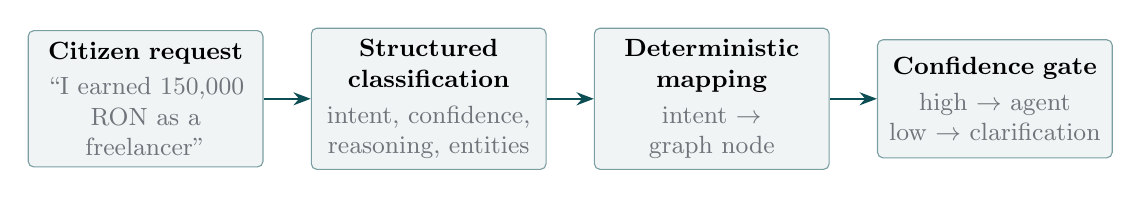
\begin{tikzpicture}[node distance=6mm, every node/.style={font=\small},
      box/.style={draw=teal!55, fill=teal!6, rounded corners=2pt, align=center,
                  inner sep=4pt, text width=27mm, minimum height=15mm},
      ar/.style={-{Stealth[length=2.2mm]}, draw=teal, line width=0.8pt}]
    \node[box] (q) {\textbf{Citizen request}\\[2pt]\cmt{``I earned 150,000 RON as a freelancer''}};
    \node[box, right=of q] (c) {\textbf{Structured classification}\\[2pt]\cmt{intent, confidence, reasoning, entities}};
    \node[box, right=of c] (m) {\textbf{Deterministic mapping}\\[2pt]\cmt{intent $\rightarrow$ graph node}};
    \node[box, right=of m] (g) {\textbf{Confidence gate}\\[2pt]\cmt{high $\to$ agent\\low $\to$ clarification}};
    \draw[ar] (q) -- (c); \draw[ar] (c) -- (m); \draw[ar] (m) -- (g);
  \end{tikzpicture}
  \end{center}
  \vfill
  \begin{itemize}
    \item The LLM classifies; it does not decide the route. A fixed table turns the predicted
      intent into a graph node, so the routing step itself can be inspected.
    \item Below the confidence threshold the request goes to clarification, even when an intent
      was assigned. Dispatching the wrong specialist here means \hl{computing the wrong tax}.
  \end{itemize}
\end{frame}

\begin{frame}{The fault injector}
  \begin{columns}[c]
    \begin{column}{0.46\textwidth}
      \begin{block}{Mechanism}
        \small A decorator wraps each simulated government boundary. \hl{One Bernoulli draw per
        call} decides whether a fault fires; if it does, exactly one operator is applied, drawn
        uniformly, so each accounts for a quarter of injected faults. Every event is logged
        with the operation and the operator type.
      \end{block}
      \begin{block}{Parameters}
        \small
        $s$: seed, for deterministic replay\\
        $\eta$: per-call injection rate\\
        $\Delta t_{\max}$: bound on the induced delay\\[0.3em]
        At $\eta = 0$ the nominal system is recovered unchanged.
      \end{block}
    \end{column}
    \begin{column}{0.50\textwidth}
      \small
      \begin{tabular}{@{}ll@{}}
        \toprule
        \textbf{Operator} & \textbf{Effect on the call}\\
        \midrule
        Timeout    & raises \texttt{TimeoutError}, no payload\\
        Delay      & sleeps up to $\Delta t_{\max}$, payload intact\\
        Partial    & one field set to \texttt{None}\\
        Corruption & one field replaced by a sentinel\\
        \bottomrule
      \end{tabular}
    \end{column}
  \end{columns}
\end{frame}

\begin{frame}{Injection decision flow}
  \vspace{-1mm}
  \centering
  \includegraphics[width=\textwidth, height=0.87\textheight, keepaspectratio]%
                  {fault-injection-flow.png}
\end{frame}

\begin{frame}{Why the faults are silent}
  Agent control flow usually turns on a single field: a predicate such as
  \texttt{status == "success"}. The rest of the response object carries content the branch
  never inspects.
  \vfill
  \begin{center}
  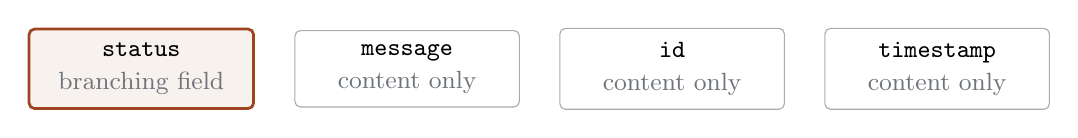
\begin{tikzpicture}[every node/.style={font=\small},
      f/.style={draw=stone!60, fill=white, rounded corners=2pt, align=center,
                inner sep=5pt, text width=25mm},
      gate/.style={draw=rust, fill=rust!7, line width=1pt}]
    \node[f, gate] (s) {\texttt{status}\\[1pt]\cmt{branching field}};
    \node[f, right=5mm of s] (m) {\texttt{message}\\[1pt]\cmt{content only}};
    \node[f, right=5mm of m] (i) {\texttt{id}\\[1pt]\cmt{content only}};
    \node[f, right=5mm of i] (t) {\texttt{timestamp}\\[1pt]\cmt{content only}};
  \end{tikzpicture}
  \end{center}
  \vfill
  \begin{columns}[T]
    \begin{column}{0.44\textwidth}
      A single-field perturbation that misses \texttt{status} leaves the predicate true, so the
      agent takes the success branch anyway. For a response with $|\mathcal{F}|$ fields whose
      branch reads exactly one of them:
      \[ P(\text{silent}) = 1 - \frac{1}{|\mathcal{F}|} \]
      The response above has four fields, so a hit misses \texttt{status} three times in four.
    \end{column}
    \begin{column}{0.52\textwidth}
      \vspace*{-1.1em}
      \begin{block}{Expected silent rate}
        \centering
        {\footnotesize
        \begin{tabular}{@{}lccr@{}}
          \toprule
          \textbf{Operator} & \textbf{Share} & \textbf{Silent} & \textbf{Contributes}\\
          \midrule
          Timeout    & 0.25 & 0    & 0\\
          Delay      & 0.25 & 1    & 0.2500\\
          Partial    & 0.25 & 0.75 & 0.1875\\
          Corruption & 0.25 & 0.75 & 0.1875\\
          \midrule
          \multicolumn{3}{@{}l}{\textbf{Expected silent rate}} & \risk{0.625}\\
          \bottomrule
        \end{tabular}}
        \\[0.4em]
        {\color{stone}\scriptsize Operators are drawn uniformly, so each is a quarter of
        injected faults. Delay preserves the payload, timeout always raises, and partial and
        corruption miss \texttt{status} with probability $0.75$.}
      \end{block}
    \end{column}
  \end{columns}
\end{frame}

%% ============================================================== PART 3 ======
\keypart{PART 3}{Evaluation}
\section{Evaluation}

\begin{frame}{Experimental setup}
  \begin{columns}[T]
    \begin{column}{0.48\textwidth}
      \begin{block}{Prototype}
        \small Python 3.11, LangGraph 0.2, GPT-4o, running on the UiPath platform. Government
        calls run against a boundary layer that reproduces the portal schemas, so no live portal
        traffic is required.
      \end{block}
      \begin{block}{Runs}
        \small $N = 100$ boundary calls, each an independent trial with at most one injected
        fault, sampled across the 8 portal-facing operations by call frequency in the five
        demo workflows.\\[0.3em]
        $\eta \in \{0,\ 0.25,\ 0.50,\ 0.75,\ 1.00\}$, \quad $s = 17$, \quad
        $\Delta t_{\max} = 250$\,ms.
      \end{block}
    \end{column}
    \begin{column}{0.48\textwidth}
      \begin{block}{Detectable}
        \small The response signals failure: an exception propagates, or an explicit error or
        degraded-service notice reaches the user.
      \end{block}
      \begin{alertblock}{Silent pass-through}
        \small Everything else counts as silent: the citizen-facing answer looks normal.
      \end{alertblock}
      \medskip
      \cmt{The unit of analysis is the call, not the session. A full workflow crosses several
      boundaries, each with its own draw.}
    \end{column}
  \end{columns}
\end{frame}

\begin{frame}{A complete trace}
  \begin{columns}[T]
    \begin{column}{0.48\textwidth}
      A citizen reports PFA income of 150,000 RON and asks what contributions are owed.
      \begin{enumerate}\small
        \item Entry Agent classifies \texttt{pfa\_d212\_filing} with confidence 0.95
        \item PFA Agent computes CAS and CASS and asks for confirmation
        \item On the confirmation turn the SPV submission call is intercepted at
          $\eta = 1.0$, $s = 17$
      \end{enumerate}
      \medskip
      {\scriptsize\ttfamily\color{rust}
       [WARN] fault injected | op=mock\_spv\_submit\_d212 | type=partial}
    \end{column}
    \begin{column}{0.48\textwidth}
      The \texttt{message} field of \texttt{SPVSubmissionResult} was set to \texttt{None}.
      \texttt{status} stayed \texttt{"success"}, so the agent followed the success branch and
      answered:
      \medskip
      \begin{alertblock}{What the citizen saw}
        \small\emph{``The D212 declaration was successfully submitted!
        ID: D212-01B66C85C3, Timestamp: 2026-03-27T22:20:32.''}
      \end{alertblock}
      \medskip
      \cmt{The response has four fields and the branch reads only one of them, so a fault that
      hits a single field goes unnoticed with probability $0.75$. The same arithmetic applies
      to any response whose branch reads one field.}
    \end{column}
  \end{columns}
\end{frame}

\begin{frame}{Fault injection results}
  \begin{table}
    \small
    \begin{tabular}{@{}rrrrrrrr@{}}
      \toprule
      $\eta$ & Faults & TO & DL & PT & CR & Silent & Detectable\\
      \midrule
      0.00 & 0   & 0  & 0  & 0  & 0  & 0 (n/a) & 0 (n/a)\\
      0.25 & 25  & 6  & 6  & 7  & 6  & 16 (64\%) & 9 (36\%)\\
      0.50 & 50  & 12 & 13 & 12 & 13 & 32 (64\%) & 18 (36\%)\\
      0.75 & 75  & 19 & 19 & 18 & 19 & 47 (63\%) & 28 (37\%)\\
      1.00 & 100 & 25 & 25 & 25 & 25 & \risk{63 (63\%)} & 37 (37\%)\\
      \bottomrule
    \end{tabular}
    \\[0.4em]
    \cmt{$N = 100$ calls, $s = 17$, $\Delta t_{\max} = 250$\,ms.
    TO, DL, PT, CR: timeout, delay, partial, corruption.}
  \end{table}
  \vfill
  \begin{itemize}
    \item The measured rate matches the predicted \risk{0.625}. Raising $\eta$ raises the
      \emph{count} of silent faults, but the proportion does not move.
    \item Delay leaves the payload intact, so it is silent by construction. It is also
      imperceptible: even at $\eta = 0.50$ it adds around 65\,ms to a whole scenario.
    \item The same arithmetic carries to other agents: wherever a branch turns on one field,
      the exposure follows from the response schema, and \hl{widening what the branch inspects
      is what lowers it}.
  \end{itemize}
\end{frame}

\begin{frame}{Cost feasibility}
  \begin{columns}[T]
    \begin{column}{0.31\textwidth}
      \centering
      \textbf{Per session}\\[0.4em]
      {\Large\color{teal}\bfseries \$0.05}\\[0.4em]
      \cmt{one classification, two to three domain turns and one retrieval step}
    \end{column}
    \begin{column}{0.31\textwidth}
      \centering
      \textbf{Small office}\\[0.4em]
      {\Large\color{teal}\bfseries \$51}\\[0.4em]
      \cmt{per month, 50 sessions a day}
    \end{column}
    \begin{column}{0.31\textwidth}
      \centering
      \textbf{Large agency}\\[0.4em]
      {\Large\color{teal}\bfseries \$5,060}\\[0.4em]
      \cmt{per month, 5,000 sessions a day}
    \end{column}
  \end{columns}
  \vfill
  \begin{itemize}\small
    \item About 20,000 input and 2,100 output tokens per session, priced at \$1.25 per million
      input and \$10.00 per million output tokens,$^{\dagger}$ over 22 working days a month.
      Licensing, infrastructure and maintenance are excluded.
    \item Cost scales linearly with volume and remains low at institutional scale. Routing with
      a smaller model and reserving the capable one for domain reasoning lowers it further.
  \end{itemize}
  \vfill
  \centering
  \hl{At these volumes, cost is not what blocks deployment. Assurance is.}
  \vfill
  \raggedright
  {\color{stone}\footnotesize $^{\dagger}$ Pricing is the GPT-5 public snapshot at the time of
   the experiment; the prototype itself runs GPT-4o. The figures indicate order of magnitude
   under an illustrative deployment scenario, not a fixed deployment cost.}
\end{frame}

%% ============================================================== PART 4 ======
\keypart{PART 4}{Conclusion}
\section{Conclusion}

\begin{frame}{Conclusion}
  \begin{block}{RQ1 \quad How much gets through?}
    \small \risk{63\%} of injected boundary faults reach the citizen with no signal: 16 of 25 at
    $\eta = 0.25$, 63 of 100 at $\eta = 1.00$. Close to two faults in every three arrive dressed
    as an ordinary success message.
  \end{block}
  \begin{block}{RQ2 \quad Incidental, or structural?}
    \small Structural. The rate is set by the operator mix and the number of fields in the
    response object, matches $0.25 + 2 \times 0.25 \times 0.75 = 0.625$ in closed form, and does
    not move with the injection rate. The branch is already correct with respect to the flag it
    reads, so the fix belongs in an \hl{output contract}, not in the branch.
  \end{block}
  \vfill
  \centering
  \hl{A coherent interface is no evidence that the execution behind it was correct.}
\end{frame}

\begin{frame}{What remains to be tested}
  \small
  The 63\% is a property of \emph{this} architecture: a fixed routing graph whose branches read
  one status field. Each item below changes something that rate depends on, and none has been
  measured yet.
  \vfill
  \begin{enumerate}\small
    \item \textbf{Output contracts and guardrails.} Validity conditions on the assembled
      response before it reaches the citizen, and schema and policy checks at the boundary
      itself: a submission identifier that must be present and well formed, a payment code that
      must match its shape. Both catch what a branching predicate structurally cannot, and how
      much each recovers is an open number.
    \item \textbf{Other agent architectures.} A \hl{ReAct loop} choosing freely among the shared
      tools, or a \hl{skill-driven agent} selecting a procedure at run time, reads different
      fields on different turns. Whether that raises detection or moves the blind spot is
      untested.
    \item \textbf{Trace-based assurance.} Message-action traces, deterministic replay and
      action-level governance, so a silent condition stays recoverable after the fact.
    \item \textbf{Realistic conditions.} Live portals in place of simulated ones, and faults
      compounding across a full session rather than one call at a time.
  \end{enumerate}
\end{frame}

%% =============================================================== thank you ==
\begin{frame}[plain, noframenumbering]
  \vfill
  \centering
  {\color{teal}\Large\bfseries Thank you}\\[0.6em]
  Questions?\\[1.4em]

  {\color{rust}\rule{0.86\paperwidth}{2pt}}\\[1.3em]

  {\small Radu-Mihai Gheorghe \quad$\cdot$\quad Petru-Liviu Bouruc \quad$\cdot$\quad
   Ciprian Paduraru \quad$\cdot$\quad Alin Stefanescu}\\[0.4em]
  {\small UiPath \quad$\cdot$\quad University of Bucharest \quad$\cdot$\quad
   Institute for Logic and Data Science}
  \vfill
\end{frame}

%% ================================================================= backup ==
\appendix
\backupslidetrue
\keypart{BACKUP SLIDES}{Additional material}

\begin{frame}[noframenumbering]{Backup: the five domain agents}
  \begin{columns}[T]
    \begin{column}{0.48\textwidth}
      \begin{block}{PFA / Freelancer}
        \small \emph{Declara\c{t}ia Unic\u{a}} (D212). Computes the pension contribution
        (CAS, 25\% on a band-stepped base) and the health contribution (CASS, 10\% of net
        income, floor $6\times$ and ceiling $72\times$ the minimum gross salary). Submission
        through SPV.
      \end{block}
      \begin{block}{Property sale}
        \small 3\% of the sale value under three years of ownership, 1\% at three years or
        more. Payment guidance through Ghi\c{s}eul.ro.
      \end{block}
      \begin{block}{Rental income}
        \small Contract registration with ANAF and a 10\% flat tax on annual rent.
      \end{block}
    \end{column}
    \begin{column}{0.48\textwidth}
      \begin{block}{Certificate}
        \small \emph{Certificat de atestare fiscal\u{a}}. It identifies the certificate type,
        checks the document requirements and guides submission.
      \end{block}
      \begin{block}{RO e-Factura}
        \small B2B and B2C invoicing: invoice data collection, XML generation to the national
        standard, submission and status monitoring.
      \end{block}
      \medskip
      \cmt{All five produce a standardised response field from the final model output, which
      keeps the formatting consistent across workflows.}
    \end{column}
  \end{columns}
\end{frame}

\begin{frame}[noframenumbering]{Backup: the four shared services}
  \begin{columns}[T]
    \begin{column}{0.48\textwidth}
      \begin{block}{Document intake}
        \small OCR plus validation against document-specific schemas for D212 forms, rental
        contracts and invoices. Returns structured data with confidence scores; below 80\%
        the document is flagged for manual review.
      \end{block}
      \begin{block}{RAG}
        \small Retrieval over dedicated indices of the Romanian Tax Code and procedural
        guidance, so every answer can be traced to a passage in the law and none of it rests
        on what the model happens to remember.
      \end{block}
    \end{column}
    \begin{column}{0.48\textwidth}
      \begin{block}{Calculation}
        \small All arithmetic is decimal, never floating point. Rates and thresholds
        (minimum salary, contribution percentages) are read from configuration, so annual
        regulatory updates need no code change.
      \end{block}
      \begin{block}{Payment}
        \small Builds the payment request from the shared context, initiates it through
        Ghi\c{s}eul.ro and returns the transaction details, including the redirect URL.
      \end{block}
    \end{column}
  \end{columns}
  \vfill
  \cmt{The division of labour is the same in all four: the model interprets the request,
  deterministic code performs the computation.}
\end{frame}

\begin{frame}[noframenumbering]{Backup: where the work sits}
  \begin{columns}[T]
    \begin{column}{0.31\textwidth}
      \textbf{Agentic orchestration}\\[0.3em]
      \cmt{LangGraph models control flow as a typed state machine. Each transition is
      explicit and can be audited. That matters when the service is regulated.}
    \end{column}
    \begin{column}{0.31\textwidth}
      \textbf{Retrieval}\\[0.3em]
      \cmt{Tax law is specific and amended often. Retrieval grounds explanations in the
      Romanian Tax Code and is kept separate from the deterministic computation.}
    \end{column}
    \begin{column}{0.31\textwidth}
      \textbf{Chaos engineering}\\[0.3em]
      \cmt{Faults are introduced deliberately and their effects observed. The technique reached
      LLM agents recently, though mostly in generic or synthetic testbeds.}
    \end{column}
  \end{columns}
  \vfill
  \begin{block}{Closest neighbours}
    \small Work on faults in agentic repositories identifies the boundary between probabilistic
    model output and deterministic program logic as a dominant failure class. That is the same
    interface targeted here. Reliability benchmarks for LLM agents include timeout,
    partial-response and schema-drift conditions, but do not connect the observed silent rate
    to schema structure in a deployed public-service setting.
  \end{block}
\end{frame}

\begin{frame}[noframenumbering]{Backup: cost model}
  \begin{table}
    \small
    \begin{tabular}{@{}lrrr@{}}
      \toprule
      \textbf{Institution size} & \textbf{Sessions/day} & \textbf{Sessions/month} & \textbf{Cost/month}\\
      \midrule
      Small office  & 50    & 1,100   & \$51\\
      Medium office & 500   & 11,000  & \$506\\
      Large agency  & 5,000 & 110,000 & \$5,060\\
      \bottomrule
    \end{tabular}
    \\[0.4em]
    \cmt{22 working days per month; \$1.25 per 1M input and \$10.00 per 1M output tokens.}
  \end{table}
  \vfill
  \begin{itemize}\small
    \item Per session: one Entry Agent call ($\approx$ 2,000 input / 200 output tokens),
      two to three domain turns ($\approx$ 5,000 / 500 each), one retrieval-grounded step
      ($\approx$ 3,000 / 400). About 20,000 input and 2,100 output tokens in total.
    \item Costs scale at roughly \$1.01 per daily session per month.
    \item The prototype runs GPT-4o; the projection uses the pricing of a stronger model as an
      illustrative deployment scenario.
  \end{itemize}
\end{frame}

\begin{frame}[noframenumbering]{Backup: reproducibility}
  \begin{columns}[T]
    \begin{column}{0.48\textwidth}
      \begin{block}{Deterministic replay}
        \small The injector draws from a seeded generator, so a fixed $(s, \eta,
        \Delta t_{\max})$ reproduces the same sequence of operators over the same sequence of
        boundary calls. Runs reported here use $s = 17$.
      \end{block}
      \begin{block}{Fault log}
        \small Each injected event is written as a warning naming the operation and the
        operator, which is what makes the qualitative trace on the earlier slide checkable:\\[0.3em]
        {\scriptsize\ttfamily [WARN] fault injected | op=... | type=...}
      \end{block}
    \end{column}
    \begin{column}{0.48\textwidth}
      \begin{block}{Calibration}
        \small Delay sleeps for a draw from $\mathcal{U}[1, \Delta t_{\max}]$. Measured across
        affected calls: $125.5 \pm 72.2$\,ms, against 125.5 and 71.9 predicted for
        $\mathcal{U}[1,250]$, so the operator draws from the interval it claims.
      \end{block}
      \begin{block}{Turning injection off}
        \small Setting $\eta = 0$ returns every payload unchanged, so the same code path serves
        both the nominal system and the perturbed one. The injector never modifies the
        portal stub logic itself.
      \end{block}
    \end{column}
  \end{columns}
\end{frame}

\end{document}
